\documentclass[final,xcolor=dvipsnames]{beamer}
%
% Choose how your presentation looks.
%
% For more themes, color themes and font themes, see: 
% http://deic.uab.es/~iblanes/beamer_gallery/index_by_theme.html
%

%the-sun-is-in-love-with-the-moon-collab-with-blaak.jpg

\graphicspath{{./Figs/}}


\mode<presentation>
{
  \usetheme{Boadilla}      % or try Darmstadt, Madrid, Warsaw, ...
  \usecolortheme{default} % or try albatross, beaver, crane, ...
  \usefonttheme{structurebold}  % or try serif, structurebold, ...
  \setbeamertemplate{navigation symbols}{}
  \setbeamertemplate{caption}[numbered]
} 

\usepackage[english]{babel}
\usepackage[utf8x]{inputenc}
\usepackage[]{caption}
\usepackage{tikz}
\usepackage[dvipsnames]{xcolor}

\usepackage{phaistos}

%% Section name as title %%% 
\addtobeamertemplate{frametitle}{\let\insertframetitle\insertsubsectionhead}{}
%\addtobeamertemplate{frametitle}{\let\insertframesubtitle\insertsectionhead}{}
\makeatletter
\CheckCommand*\beamer@checkframetitle{\@ifnextchar\bgroup\beamer@inlineframetitle{}}
\renewcommand*\beamer@checkframetitle{\global\let\beamer@frametitle\relax\@ifnextchar\bgroup\beamer@inlineframetitle{}}
\makeatother
%% %% %% %% 

%\titlegraphic{\includegraphics[]{the-sun-is-in-love-with-the-moon-collab-with-blaak.jpg} \hspace{2cm} \includegraphics[width=2cm]}}
\title[Introduction to Environmental Modelling]{Introduction to Environmental Modelling}
\subtitle{Face-It Summer School 2019 : Marine Biogeochemical Cycling: from measurements to modelling}
\author[A. Capet]{A. Capet, M.Grégoire, K. Soetaert} %Logo de MAST +logo interface sur chaque slide et page de garde interface?
\institute[http://labos.ulg.ac.be/mast/]{MAST - acapet@ulg.ac.be}
\date[Oct 2019]

%\AtBeginSubsection[]{
%  \begin{frame}
%  \vfill
%  \centering
%  \begin{beamercolorbox}[sep=8pt,center,shadow=true,rounded=true]{title}
%    \usebeamerfont{title}\insertsectionhead\par%
%    \usebeamerfont{title}\insertsubsectionhead\par%
%  \end{beamercolorbox}
%  \vfill
%  \end{frame}
%}

\AtBeginSubsection[]{
  \frame<beamer>{ 
    \frametitle{Outline}   
    \tableofcontents[currentsection,currentsubsection] 
  }
}

\begin{document}
  \def\mussel{\PHoxBack}
  \def\extitle[#1]{\centering{ \mussel \hspace{2cm} #1 \hspace{2cm} \mussel}}
  \def\unit[#1]{$\mathrm{#1}$}
  \def\parC[#1]{\textcolor{Blue}{#1}}
  \def\proC[#1]{\textcolor{Green}{#1}}
  \def\varC[#1]{\textcolor{Red}{#1}}
  \def\worC[#1]{\textcolor{Orange}{#1}}
  \def\forC[#1]{\textcolor{Aquamarine}{#1}}
  % \usebackgroundtemplate{%             declare it
  % \tikz[overlay,remember picture] \node[opacity=0.6, at=(current page.center)] {
  %   \includegraphics[height=\paperheight,width=\paperwidth]{the-sun-is-in-love-with-the-moon-collab-with-blaak.jpg}
  %   };
  %   % {Great_Barrier_Reef_Australia}};
  % }
  
  \begin{frame}
    \titlepage
  \end{frame}
  
  % \usebackgroundtemplate{ }  
  
  \section{Basics Concepts}
  \subsection{What is a model ?}
  \begin{frame}
    What is a model ? \\
    \visible<2->{
      \center{ A \alert{simplified} representation of a complex phenomenon.}\\} 
      \visible<3->{
	\flushleft What are models used for?}
      \only<4>{
	\begin{itemize}
	  \item Understand Observations:
	  \begin{itemize}
	    \item Confront Theory to Observations, ie. check hypotheses
	    \item Unified framework
	  \end{itemize}
	  \item Complete Observations : 
	  \begin{itemize}
	    \item Upscale Observations 
	    \item Quantify processes difficult to measure 
	  \end{itemize}
	  \item Assess Scenarios  % Management
	  \begin{itemize}
	    \item Management
	    \item Predict the Future (or attempt to)
	    \item Reconstruct the Past 
	  \end{itemize}
	\end{itemize}
      }
      \visible<5->{
	%\pause 
	\center{ 
	  Understand-Quantify / Complete / Predict / Assess %.}
	  \\} 
	}
      \end{frame}
      
      \begin{frame}
	How \alert{simple} should a model be ? \\
	\pause 
	\vspace{1cm}
	\textit{\Large ``As simple as possible, but not simpler''} [A. Einstein]\\
		\vspace{1cm}
	\pause
	\centering{Arguments in favor of:}
	\begin{columns}
	  \begin{column}{.5\framewidth}
	    \centering{\alert{Simplicity}}\\
	    \visible<3->{
	      \begin{itemize}
		\item Computation Time
		\item Facility of Analysis, description
		\item Occam's Razor 
		\item Lack of knowledge / Observations
	      \end{itemize}}
	  \end{column}
	  \begin{column}{.5\framewidth}
	    \centering{\alert{Complexity}}\\
	    \visible<3->{ \begin{itemize}
		\item Realism
		\item Accuracy
		\item Inner 'local' mechanisms support system 'global' properties
	      \end{itemize}
	    }
	  \end{column}
	\end{columns}
      \end{frame}
      
      \subsection{Type of models}
      \begin{frame}
	\framesubtitle{Statistical Models}
	\begin{columns}
	  \begin{column}{.5\framewidth}
	    \begin{itemize}
	      \item Basis : Observations \& Statistics
	      \item Example: Species Distribution modelling
	      \item Hypothesis : environmental conditions act as
	      the first filter to determine species distribution.
	      \item Expressed as : Calibrated relationships.
	      \item Use : Predict species distribution in unsampled sites 
	      \item Limitation : Extrapolation outside of obs. range ? 
	    \end{itemize}
	  \end{column}
	  \begin{column}{.5\framewidth}
	    \begin{figure}
	      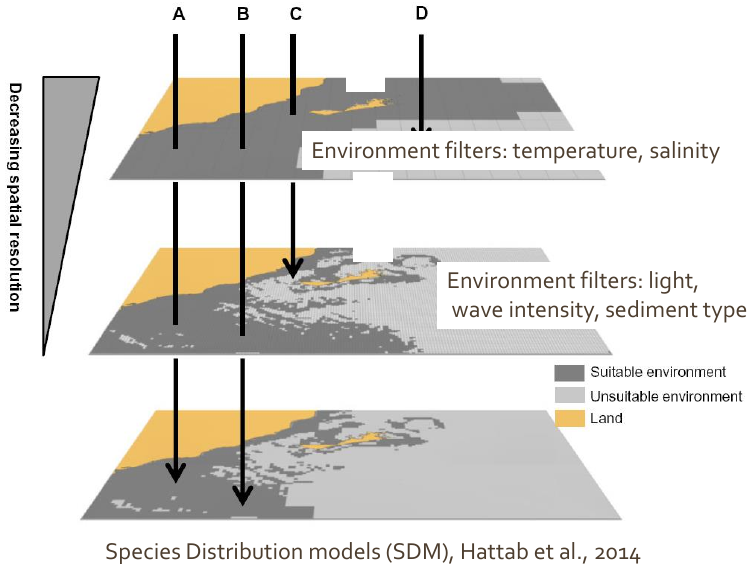
\includegraphics[width=.95\columnwidth]{SDM}
	    \end{figure}
	  \end{column}
	\end{columns}
      \end{frame}
      
      \begin{frame}
	\framesubtitle{Mechanistic Models}
	\begin{columns}
	  \begin{column}{.8\framewidth}
	    \begin{itemize}
	      \item Basis : Knowledge on Processes
	      \item Example: Meteo, Ocean circulation, growth, etc ..
	      \item Hypothesis : Mechanisms and interactions does not changes, and rules the evolution of the system. 
	      \item Expressed as : (Often) Set of differential equations
	      \item Use : Understand, Forecast, Scenario.
	      \item Limitation : Demanding, needs loads of simplification, assumptions .. 
	    \end{itemize}
	  \end{column}
	  \begin{column}{.2\framewidth}
%	    \begin{figure}
%	      \includegraphics[width=.95\columnwidth]{}
%	    \end{figure}
	  \end{column}
	\end{columns}
      \end{frame}
      
      
      \subsection{Building a model}
      \begin{frame}
	% XXX Decompose into Steps with partial figures. 
	\begin{figure}
	  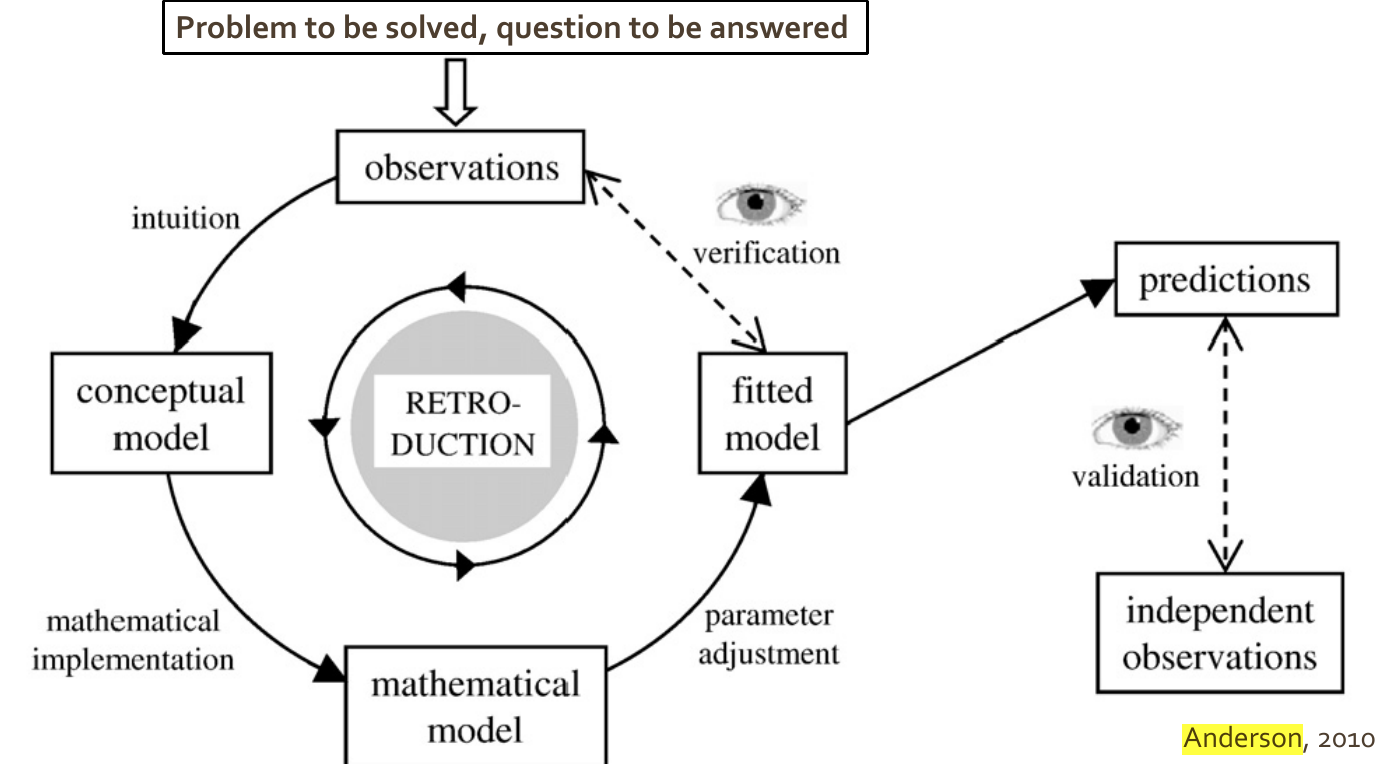
\includegraphics[width=.95\columnwidth]{ModellingSteps}
	\end{figure}
      \end{frame}
      
      \section{Conceptual model}
      \subsection{Research Questions}
      
      \begin{frame}
	\begin{block}{Research Questions}
	  \begin{itemize}
	    \item Clear formulation of the research question should lead decisions for all elements of the model 
	  \end{itemize}
	\end{block}
      \end{frame}
      
      \begin{frame}
	\begin{exampleblock}{\extitle[Research Context]}
	  \begin{columns}
	    \begin{column}{0.5\framewidth}
	      \begin{figure}
		\centering
		
\includegraphics[width=.9\columnwidth]{./Figs/Context.png}
		%\caption{Caption}
		\label{fig:my_label}
	      \end{figure}
	    \end{column}
	    \begin{column}{0.5\framewidth}
	      Our study mainly focuses on 
	      \begin{itemize}
		\item increased production of organic matter (faeces and pseudofaeces)
		\item food depletion by the growth of biofouling %organisms
		\item impacts on biogeochemical processes via respiration and excretion. 
	      \end{itemize}
	    \end{column}
	  \end{columns}
	\end{exampleblock}
      \end{frame}
      
      \begin{frame}
	\begin{exampleblock}{\extitle[Research Questions]}
	  \begin{itemize}
	    \item How \alert<2>{deep} can the blue mussels grow under \alert<2>{mixed/stratified} conditions,
	    \item Will there be local \alert<2>{depletion of food resources} such as phytoplankton, zooplankton and detritus ?
	    \item Will mussels on \alert<2>{seabed} have the same effect as mussel on the structure ? 
	    \item Does type of turbine and \alert<2>{distance} between them impacts on the accumulation of mussel biomass and on ecosystem and \alert<2>{biogeochemical dynamics} ?
	  \end{itemize}
	\end{exampleblock}
      \end{frame}
      
      \subsection{Scales}
      \begin{frame}
	\begin{block}{Spatial Scales}
	  \begin{itemize}[<+->]
	    \item Relevant scales for system dynamics ?
	    \item Relevant scale for operating processes ?
	    \item Non-linearities ?
	    \item Anisotropy? In forcings ? in processes ?
	    \item Length scale of spatial resolution for available observations ?
	    \item Memory ! 
	  \end{itemize}
	\end{block}
      \end{frame}
      
      \begin{frame}
	\begin{exampleblock}{\extitle[Spatial Scales]}
	  \begin{itemize}
	    \item 1-dimension
	    \item 25 m pylone
	    \item 50 layers of 0.5 m each
	    \item<2> Horizontal length scales: characterized with parameters
	  \end{itemize} 
	  \begin{figure}
	    \centering
	    \includegraphics<2>[width=0.3\framewidth]{Figs/HorizontalL.png}
	    \label{fig:HL}
	  \end{figure}
	\end{exampleblock}
      \end{frame}
      
      \begin{frame}
	\begin{block}{Temporal Scales}
	  \begin{itemize}[<+->]
	    \item Relevant scales for system dynamics
	    \item Relevant scale for operating processes
	    \item Non-linearities
	    \item Periodicity in forcings ?  
	    \item CPU ! 
	  \end{itemize}
	\end{block}
	
      \end{frame}
      
      \begin{frame}
	\begin{exampleblock}{\extitle[Temporal Scales]}
	  \begin{itemize}[<+->]
	    \item Seasonal Temperature Cycle
	    \item Typical rates: Day $\rightarrow$ Weeks
	    \item[$\rightarrow$] Simulations of a few years, timestep of 1 day.
	  \end{itemize}
	\end{exampleblock}
      \end{frame}
      
      \subsection{State Variables}
      \begin{frame}
	\begin{block}{State variables}
	  \begin{itemize}
	    \item State variables define the state of our simplified system, at any time. 
	    \item Those are the descriptors for which we have to provide 'Rules of evolution`, 
	    in the form of differential equation.% XXX get this for mathematical model form.  $\frac{d C}{dt}=\ldots$
	    \item Usually, those rules are derived from mass conservation principles
	    \item[$\rightarrow$] State Variables needs to be expressed in a common conservative currency.
	  \end{itemize}
	\end{block}
      \end{frame}
      \begin{frame}
	\begin{exampleblock}{\extitle[State variables]}
	  \begin{columns}
	    \begin{column}{0.5\framewidth}
	      3 Components: 
	      \begin{itemize}
		\item \textbf<2>{Physics}
		\only<2>{
		  \begin{itemize}
		    \item No feed backs from others
		    \item[$\rightarrow$] Can remains external
		  \end{itemize}
		}
		\item \textbf<3-5>{Biogeochemistry}
		\only<3-5>{
		  \begin{itemize}
		    \item NPZD Approach  %XXX ILLUSTRATE NPZD
		    \item Only N limits growth. 
		    \item[$\rightarrow$] Currency: [$\mathrm{mmolN\,m^{-3}}$]
		    \item<5> \begin{itemize}
		      \item \textcolor{blue}{Inorganic}
		      \item \textcolor{green}{Living Organic}
		      \item \textcolor{red}{Dead Organic} % XX Nice colors % XX Domains
		    \end{itemize}
		  \end{itemize}
		}
		\item \textbf<6>{Mussels}
		\only<6->{ % find better symbol for ATTENTION
		  \begin{itemize}
		    \item ! Different domains !
		    \item[$\rightarrow$] Need to convert Biomass on pylons 
		    \item[$\rightarrow$] [$\mathrm{ind\,m^{-2}}$] $\rightarrow$ [$\mathrm{mmolN\,m^{-3}}$]
		  \end{itemize}
		}
	      \end{itemize}
	    \end{column}
	    \begin{column}{0.5\framewidth}
	      \only<1-2>{ 
		\begin{figure}
		  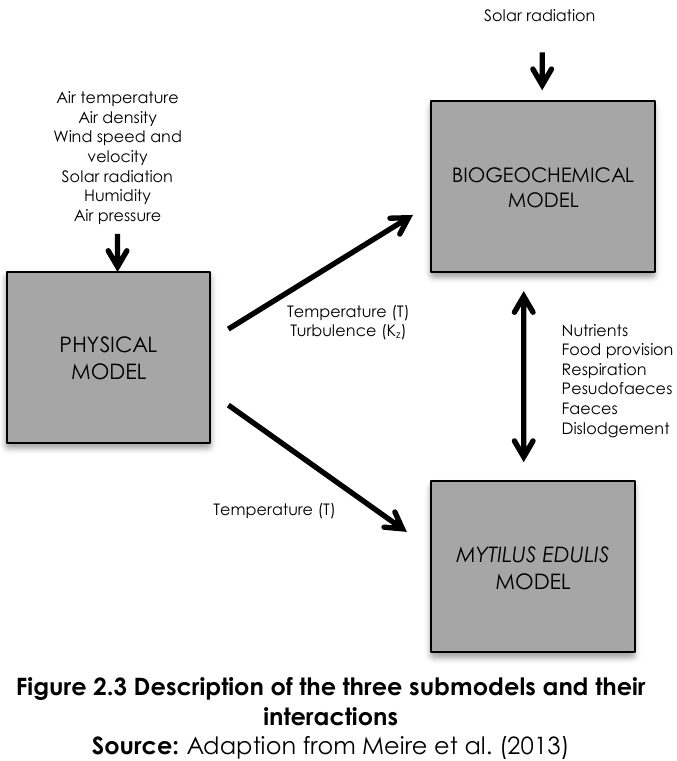
\includegraphics[width=.95\columnwidth]{3models}
		\end{figure} 
	      } 
	      \only<4-5>{ 
		\begin{itemize}
		  \item \textcolor<5>{blue}{ammonium: $\mathrm{NH4}$}
		  \item \textcolor<5>{blue}{nitrate: $\mathrm{NO3}$}
		  \item \textcolor<5>{green}{phytoplankton: $\mathrm{PHYTO}$}
		  \item \textcolor<5>{green}{zooplankton: $\mathrm{ZOO}$}
		  \item \textcolor<5>{red}{detr.: $\mathrm{PELDETRITUS}$}
		  \item \textcolor<5>{red}{bot. detr.: $\mathrm{BOTDETRITUS}$}
		\end{itemize} 
	      }
	      \only<6->{ 
		\begin{figure}
		  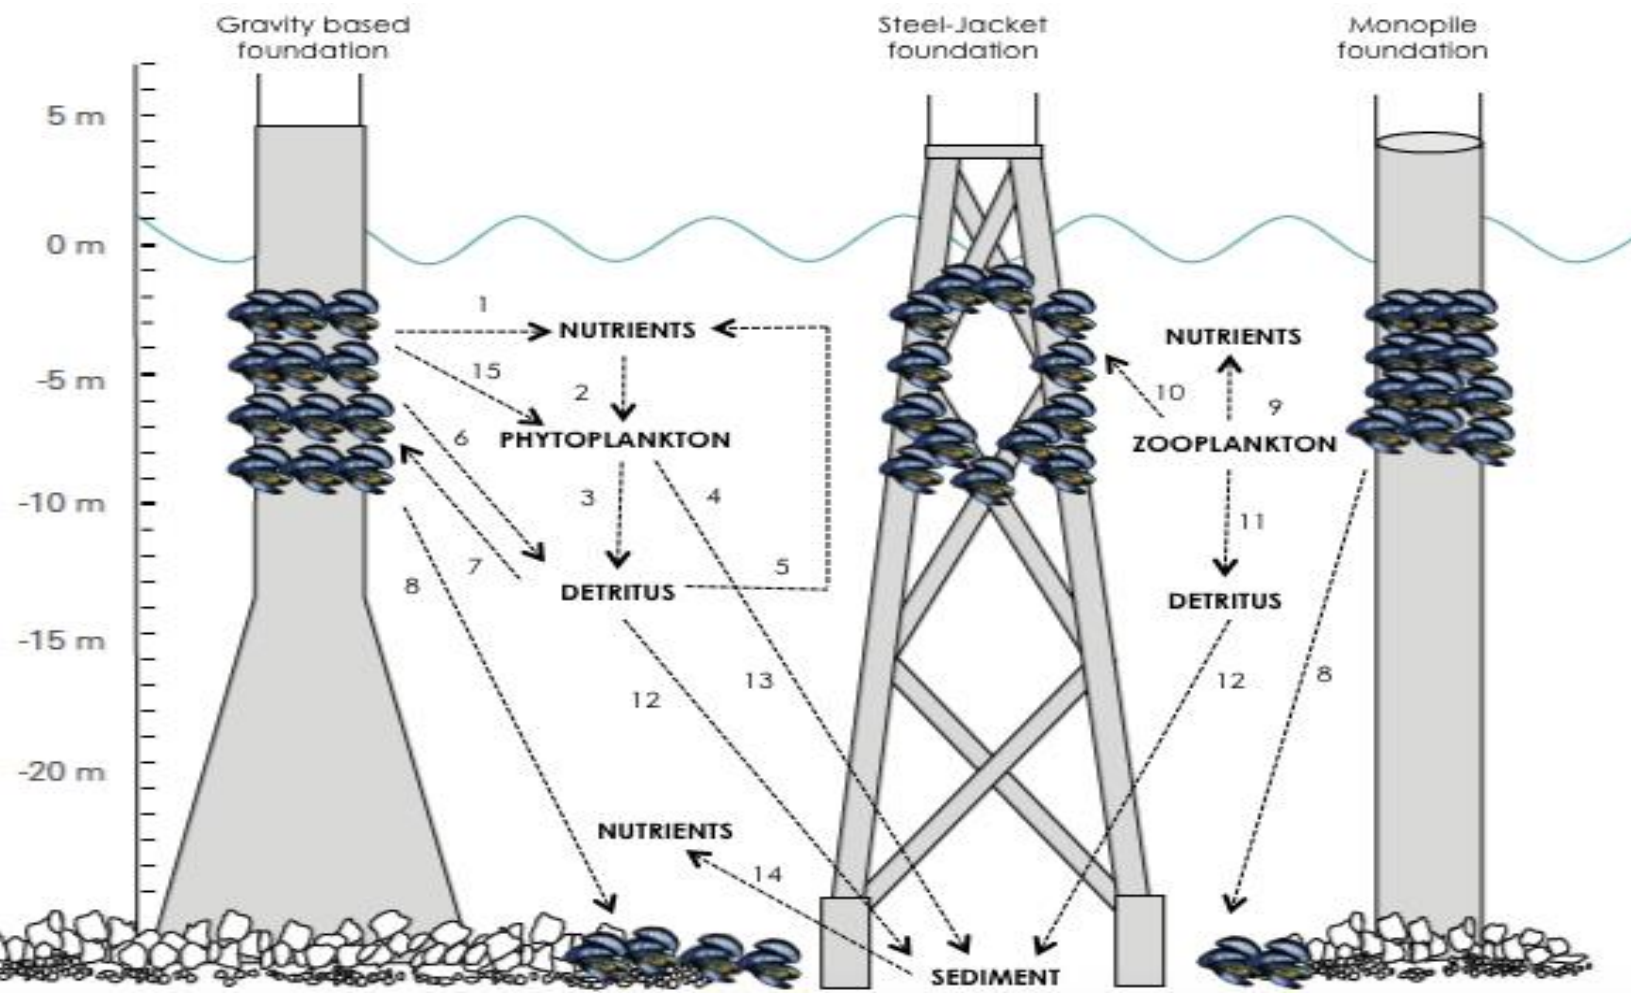
\includegraphics[width=.95\columnwidth]{Domains}
		\end{figure} 
	      } 
	    \end{column}
	  \end{columns}
	\end{exampleblock} 
      \end{frame}
      
      \subsection{Processes \& Flows}
      \begin{frame}
	\begin{block}{Mass Balance Equation}
	  \begin{itemize}
	    \item Connect Flows among state variables
	    \item Identify controls on those flows
	  \end{itemize} 
	\end{block}
      \end{frame}
      
      \begin{frame}
	\begin{exampleblock}{\extitle[Flows]}
	  \begin{columns}
	    \begin{column}{0.35\framewidth}
	      \only<1>{
		\textbf{Phytoplankton}
		\begin{itemize}
		  \item Uptake Nutrients for Growth
		  \begin{itemize}
		    \item NH3 and NO3
		    \item NH3 first
		    \item Light limitation (depth)
		  \end{itemize}
		  
		  \item Sink
		  \item Die
		\end{itemize}
	      }
	      \only<2>{
		\textbf{Zooplankton}
		\begin{itemize}
		  \item Graze on Phytoplankton
		  \item Sink
		  \item Egest nutrient
		  \item Die
		\end{itemize}
	      }  \only<3>{
		\textbf{Detritus}
		\begin{itemize}
		  \item Decay
		  \item Sink
		\end{itemize}
	      }  \only<4>{
		\textbf{Mussels}
		\begin{itemize}
		  \item Excrete and respire
		  \item Produce Faeces and pseudofaeces
		  \item Graze on PHY, ZOO, DETRITUS
		  \item Fall
		  \item Die
		\end{itemize}
	      } \end{column}
	    \begin{column}{0.65\framewidth}
	      \begin{figure}
		\includegraphics<1>[width=.95\columnwidth]{StateVariables_PHY}
		\includegraphics<2>[width=.95\columnwidth]{StateVariables_ZOO}
		\includegraphics<3>[width=.95\columnwidth]{StateVariables_DET}
		\includegraphics<4>[width=.95\columnwidth]{StateVariables_MUS}
	      \end{figure} 
	    \end{column}
	  \end{columns}
	\end{exampleblock} 
      \end{frame}
      
      
      \begin{frame}
	\begin{exampleblock}{\extitle[Physical Transport]}
	  \begin{itemize}
	    \item All pelagic variable are transported by diffusion (vertically mixed).  
	    \item PHY and DETRITUS have additional vertical sinking
	  \end{itemize} 
	\end{exampleblock}
      \end{frame}      
      
      \begin{frame}
	\begin{exampleblock}{External Controls on Processes}
	  \begin{itemize}
	    \item \textcolor<2>{blue}{Temperature} affect growth and decay rates.
	    \item \textcolor<2>{blue}{Turbulent diffusion coefficient} controls vertical diffusion.
	    \item \textcolor<2>{blue}{Light} availability limits planktonic growth.
	  \end{itemize} 
	\end{exampleblock}
      \end{frame}
      
      % \begin{frame}
      % \begin{exampleblock}{Assumptions}
      % \begin{itemize}
      %     \item Only N limits phyto growth
      %     \item Both NH4 and NO3 Uptaken, but NH3 favored (limitation).
      %     \item Light limits plankton Growth  
      %     \item Liebig's law of the minimum
      %     \item Mussels feeds on Phytoplankton
      %     \item Zooplankton feeds on phytoplankton
      % \end{itemize} 
      % \end{exampleblock}
      % \end{frame}
      
      
      
      
      %       \subsection{Conservation ?}
      %       
      %       \subsection{External Inputs}
      %       \begin{frame}
      % 	
      % 	\begin{exampleblock}{Scales}
      % 	  \begin{itemize}
      % 	    \item a one-dimensional k-$\epsilon$ turbulence closure model 
      % 	    \item Temperature
      % 	    \item Current Velocity
      % 	    \item Turbulent Kinetic Energy
      % 	    \item (Salinity Constant)
      % 	  \end{itemize} 
      % 	\end{exampleblock}
      %       \end{frame}
      %       
      \section{Mathematical model formulation}
      
      \begin{frame}
	\begin{figure}
	  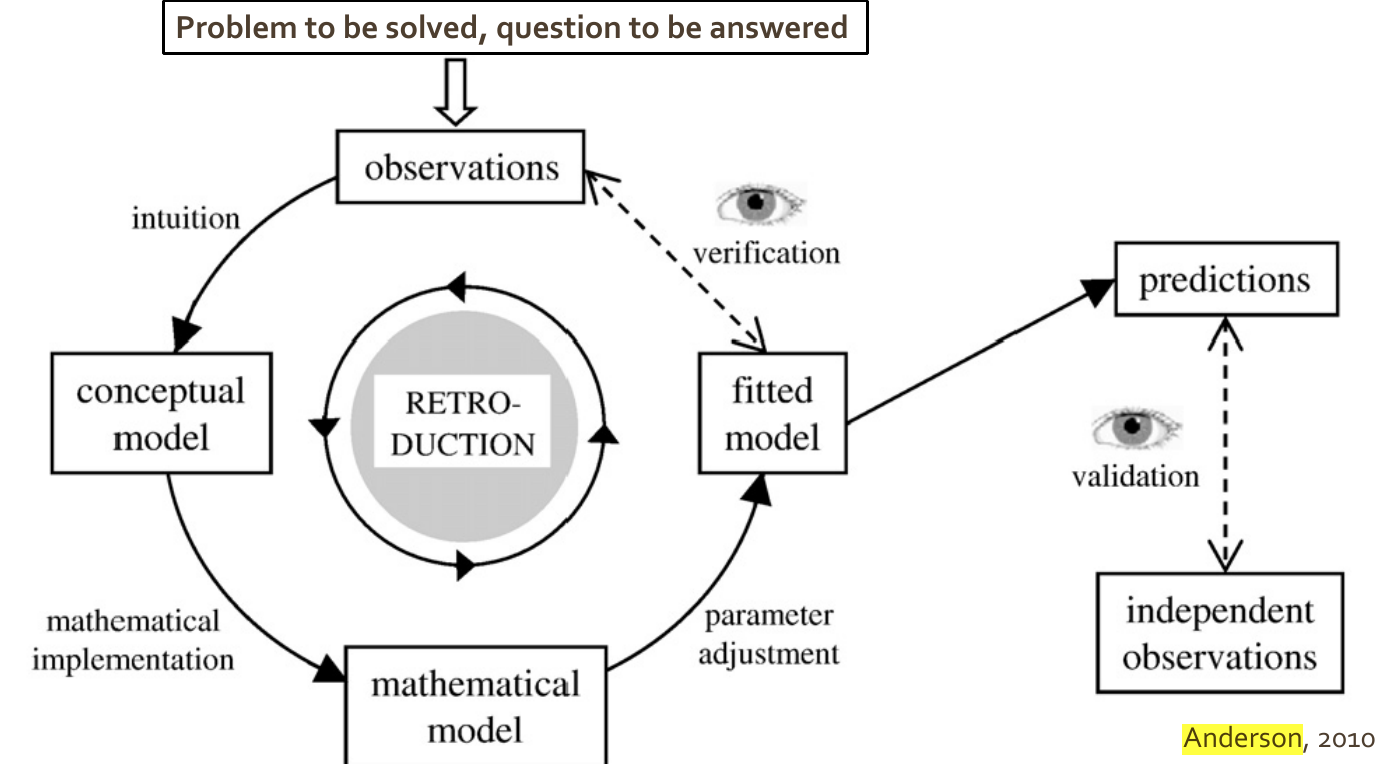
\includegraphics[width=.95\columnwidth]{ModellingSteps}
	\end{figure}
      \end{frame}
      
      
      \subsection{State Variables}
      \begin{frame}
	\begin{block}{State Vector}
	  \begin{itemize}
	    \item Spatial domain is divide in $N_{Cell}$ cells.
	    \item Sytem defined by $N_{Var}$ State Variables. 
	    \item The state of the system at time $t$, $C(t)$, can be stored numerically as a vector of size $N_{Cell}.N_{Var}$.
	  \end{itemize}
	\end{block}
	%\end{frame}
	
	
	%\begin{frame}
	\visible<2>{
	  \begin{exampleblock}{\extitle[State Vector]}
	    \begin{itemize}
	      \item NO3, NH4, PHY, ZOO, DET, and BIVALVE are defined along the vertical grid.
	      \item PELDETRITUS is defined only at the bottom.
	      \item Our state vector contains 6x50+1=301 element. 
	    \end{itemize}
	  \end{exampleblock}
	}
      \end{frame}
      
      \begin{frame}
	\begin{exampleblock}{Mussel Counts} % XX figure for detailling this
	  \begin{figure}
	    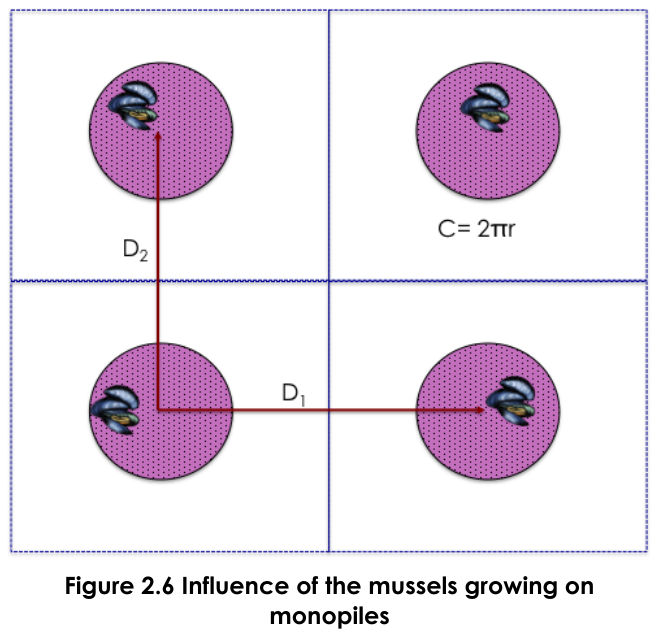
\includegraphics[width=.3\framewidth]{HorizontalL}
	  \end{figure}
	  \begin{itemize}
	    % \item Mussel lives on the surface of the windmill,
	    %\item Need to express it in terms of mmolN/m3 of surrounding water. 
	    \item Monopiles distant of $D_1$ and $D_2$, and of radius $r$. 
	    \item For a given layer ($dz$)
	    \begin{itemize}
	      \item Surface of monopile section : $2.\pi.r.dz$
	      \item Volume of water : $D_1.D_2.dz$
	    \end{itemize}
	    \item 100 \unit[mmol N\,m^{-2}] mussels on monopile $\rightarrow$ $100 x \left(\frac{2\pi r}{D_1.D_2}\right)$ \unit[mmol N\,m^{-3}] in water layer.
	  \end{itemize}
	\end{exampleblock}
      \end{frame}
      
      \subsection{Processes \& Rates}
      \begin{frame}
	\begin{block}{Equation of evolution for the State Vector}
	  \begin{itemize}[<+->]
	    \item $C(t)$ is the state vector at a given time $t$.
	    \item $\frac{\partial C}{\partial t}$ is the temporal rate of change of the state vector. 
	    \item $C(t+\Delta t) = C(t) + \frac{\partial C}{\partial t}\Delta t$ 
	    \item The equation of evolution for $C(t)$ has the form  $\frac{\partial C}{dt} = f(C,t)$ 
	  \end{itemize}
	\end{block}
      \end{frame}
      
      \begin{frame}
	\begin{block}{Transport \& Reaction}
	  \begin{figure}
	    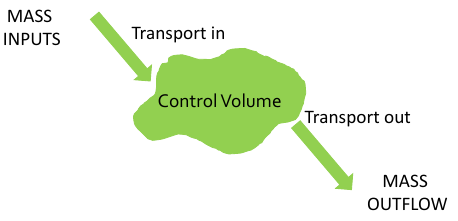
\includegraphics[width=.5\framewidth]{TransportReaction}
	  \end{figure}
	  \textbf{Transport} \visible<2>{\textbf{\& Reaction}}\\
	  $\frac{d C}{dt}$ in the control volume = $Mass\,inflow - Mass\,outflow$ \visible<2>{$\pm Reactions$}\\
	  \begin{itemize}
	    \item<3>Today, we won't deal with \alert{transport terms}, only \alert{reaction rates}
	    \item<4> We express Reaction rates through \alert{Mass Balance Equations}
	  \end{itemize}
	\end{block}
      \end{frame}
      
      
      
      \begin{frame}
	\begin{exampleblock}{\extitle[Color Code]}
	  \begin{table}
	    \begin{tabular}{ l l l}
	      Type & Unit & Example \\ \hline
	      $\varC[State\, Variable]$   & [\unit[mmol N\,m^{-3}]]          & $\varC[PHY]$ \\
	      $\proC[Processe]$        & [\unit[mmol\,N\,m^{-3}\,d^{-1}]] & $\proC[Mortality_{PHY}]$ \\ 
	      $\parC[Parameter]$       & diff.                            & $\parC[sinkingRatePhyt]$,[\unit[m\,d^{-1}]] \\
	      $\worC[Work\, Variable]$ & diff., mostly unitless           & $\worC[f(T)]$, [-] \\
	      $\forC[Forcing]$         & diff.                            & $\forC[T]$%, [$^{circle}C$] 
	    \end{tabular}
	  \end{table}
	\end{exampleblock}
      \end{frame}
      
      
      \begin{frame}
	\begin{exampleblock}{\extitle[Mass Balance Equation for PHY]}
	  \only<1>{
	    \begin{eqnarray*}
	      \small
	      \frac{\partial\,\varC[PHY]}{\partial t} & = & \proC[Diffusion_{PHY}] + \proC[Sinking_{PHY}] \\
	      & & + \proC[NPP] - \proC[Grazing_{by\,ZOO}] - \proC[Grazing_{by\,BIVAL}] - \proC[Mortality_{PHY}]
	    \end{eqnarray*}}
	  \only<2>{\begin{eqnarray*}
	      \small
	      \frac{\partial\,\varC[PHY]}{\partial t} & = & \underbrace{\proC[Diffusion_{PHY}] + \proC[Sinking_{PHY}]}_{\mathrm{Transport}} \\
	      & & + \proC[NPP] - \proC[Grazing_{by\,ZOO}] - \proC[Grazing_{by\,BIVAL}] - \proC[Mortality_{PHY}]
	    \end{eqnarray*}}
	  %   \only<3->{
	  % 	\begin{eqnarray*}
	  %      \small
	  %      \frac{\partial\,\varC[PHY]}{\partial t} & = & \proC[Diffusion_{PHY}] + \proC[Sinking_{PHY}] \\
	  %      & & + \proC[NPP] - \proC[Grazing_{by\,ZOO}] - \proC[Grazing_{by\,BIVAL}] - \proC[Mortality_{PHY}]
	  %    \end{eqnarray*}}
	\end{exampleblock}
      \end{frame} 
      
      \begin{frame}   
	\only<1>{
	\begin{exampleblock}{\extitle[Mass Balance Equation for PHY]}
	  \begin{eqnarray*}
	    \small
	    \frac{\partial\,\varC[PHY]}{\partial t} & = & \proC[Diffusion_{PHY}] + \proC[Sinking_{PHY}] \\
	    & & + \underline{\mathbf{\proC[NPP]}} - \proC[Grazing_{by\,ZOO}] - \proC[Grazing_{by\,BIVAL}] - \proC[Mortality_{PHY}]
	  \end{eqnarray*}
	\end{exampleblock}
      }
	\begin{exampleblock}{\extitle[NPP]}
	  \begin{eqnarray*}
	    \proC[NPP] &=& \parC[maxUptake].\varC[PHY].min(\worC[f(I)],\worC[f(DIN)]).\worC[f(T)]
	  \end{eqnarray*}
	  \begin{tabular}{ l l l}
	    $\parC[maxUptake]$ &  Maximum Uptake of Dissolved Inorganic Nitrogen & \unit[d^{-1}] \\
	    $ \worC[f(I)]$ & Light limitation & [-] \\
	    $ \worC[f(DIN)]$ & DIN limitation & [-] \\
	    $ \worC[f(T)]$ & Temp. effect on growth & [-] 
	  \end{tabular}
	\end{exampleblock}
	\only<2>{
	  \begin{exampleblock}{\extitle[Light limitation]}
	    \begin{equation*}
	      \worC[f(I)] = tanh \left(\frac{\forC[I(z,t)]}{\parC[I_{opt}]}    \right)
	    \end{equation*}
	    \begin{tabular}{ l l l}
	      $\forC[I(z,t)]$  & Light & \unit[W\,m^{-2}] \\
	      $\parC[I_{opt}]$ & Optimum light intensity & \unit[W\,m^{-2}] 
	    \end{tabular}
	  \end{exampleblock}
	}
	\only<3>{
	  \begin{exampleblock}{\extitle[Nutrient Limitation]}
	    \begin{equation*}
	      \worC[f(DIN)] = \frac{\varC[NO3]}{\varC[NO3] + \parC[ksNO3]}.e^{-\parC[\psi].\varC[NH3]} +  \frac{\varC[NH3]}{\varC[NH3] + \parC[ksNH3]} %XX check in R
	    \end{equation*}
	    \begin{tabular}{ l l l}
	      $\parC[ksNO3]$ &  Half-saturation coefficient for NO3 uptake & [\unit[mmol N\,m^{-3}]] \\
	      $\parC[ksNH3]$ &  Half-saturation coefficient for NH3 uptake & [\unit[mmol N\,m^{-3}]] \\
	      $\parC[\psi]$  &   Inhibition coefficient for NH4 & [\unit[mmol N^{-1}\,m^{3}]] 
	    \end{tabular}
	  \end{exampleblock}
	}
	\only<4>{
	  \begin{exampleblock}{\extitle[Temperature effect on Growth]}
	    \begin{equation*}
	      \worC[f(T)]  = \parC[Q_{10}]^{\left( \frac{\forC[T]-\parC[T_{ref}]}{10} \right) }
	    \end{equation*}
	    \begin{tabular}{ l l l}
	      $\parC[Q_{10}]$   & Temperature coefficient  & [-] \\
	      $\parC[T_{ref}]$ & Reference temperature    & [C] %[$^{\circle}C$] 
	    \end{tabular}
	  \end{exampleblock}
	}
      \end{frame} 
      
      \begin{frame}
	\begin{exampleblock}{\extitle[Mass Balance Equation for PHY]}
	  \begin{eqnarray*}
	    \small
	    \frac{\partial\,\varC[PHY]}{\partial t} & = & \proC[Diffusion_{PHY}] + \proC[Sinking_{PHY}] \\
	    & & + \proC[NPP] - \underline{\mathbf{\proC[Grazing_{by\,ZOO}]}} - \proC[Grazing_{by\,BIVAL}] - \proC[Mortality_{PHY}]
	  \end{eqnarray*}
	\end{exampleblock}
	\begin{exampleblock}{\extitle[$Grazing_{by\,ZOO}$]}
	  \begin{equation*}
	    \proC[Grazing_{by\,ZOO}] = \parC[maxGrazing] . \frac{\varC[PHY]}{\varC[PHY] + \parC[ksPHY]}.\varC[ZOO].\worC[f(T)]
	  \end{equation*}
	    \begin{tabular}{ l l l}
	      $\parC[maxGrazing]$   &  Maximum grazing rate by zooplankton  &  \unit[d^{-1}] \\
	      $\parC[ksPHY]$        & Half-saturation for zoo grazing on phyto  &  [\unit[mmol N\,m^{-3}]]
	    \end{tabular}
	\end{exampleblock}
      \end{frame}
      
            \begin{frame}
	\begin{exampleblock}{\extitle[Mass Balance Equation for PHY]}
	  \begin{eqnarray*}
	    \small
	    \frac{\partial\,\varC[PHY]}{\partial t} & = & \proC[Diffusion_{PHY}] + \proC[Sinking_{PHY}] \\
	    & & + \proC[NPP] -\proC[Grazing_{by\,ZOO}] -  \underline{\mathbf{\proC[Grazing_{by\,BIVAL}]}} - \proC[Mortality_{PHY}]
	  \end{eqnarray*}
	\end{exampleblock}
	\begin{exampleblock}{\extitle[$Grazing_{by\,BIVAL}$]}
	  \begin{equation*}
	    \proC[Grazing_{by\,BIVAL}] = \parC[maxClear] .\varC[BIVAL].\varC[PHY]. \left( 1- \frac{\varC[BIVAL]}{\parC[maxB]}\right) .\worC[f(T)]
	  \end{equation*}
	    \begin{tabular}{ l l l}
	      $\parC[maxClear]$   &   Clearance rate of the mussels  &   [\unit[mmol N\,m^{-3}\,d^{-1}] \\
	      $\parC[maxB]$       &   Carrying capacity  &  [\unit[mmol N\,m^{-3}]]
	    \end{tabular}
	    	\end{exampleblock}
      \end{frame}
      
       \begin{frame}
	\begin{exampleblock}{\extitle[Mass Balance Equation for PHY]}
	  \begin{eqnarray*}
	    \small
	    \frac{\partial\,\varC[PHY]}{\partial t} & = & \proC[Diffusion_{PHY}] + \proC[Sinking_{PHY}] \\
	    & & + \proC[NPP] -\proC[Grazing_{by\,ZOO}] -  \proC[Grazing_{by\,BIVAL}] - \underline{\mathbf{\proC[Mortality_{PHY}]}}
	  \end{eqnarray*}
	\end{exampleblock}
	\begin{exampleblock}{\extitle[$Mortality_{PHY}$]}
	  \begin{equation*}
	    \proC[Mortality_{PHY}] =  \parC[mortalityRatePhyt] . \varC[PHY] .\worC[f(T)]
	  \end{equation*}
	    \begin{tabular}{ l l l}
	      $\parC[mortalityRatePhyt]$   &   Phyto mortality rate  &   [\unit[d^{-1}]]  
	    \end{tabular}
	    \end{exampleblock}
      \end{frame}
      
      
      % NUTIRENT NO3
      \begin{frame}   
	\begin{exampleblock}{\extitle[Mass Balance Equation for NO3]}
	  \begin{eqnarray*}
	    \small
	    \frac{\partial\,\varC[NO3]}{\partial t} & = & \proC[Diffusion_{NO3}] - (1-\worC[\alpha]).\proC[NPP] + \proC[Nitrification]
	  \end{eqnarray*}
	  \begin{tabular}{ l l l }
	    $\worC[\alpha]$ & Inhibition of NO3 uptake by the presence of NH3 & [-]
	  \end{tabular}
	\end{exampleblock}
      \end{frame} 

      
      \begin{frame}   
	\begin{exampleblock}{\extitle[Mass Balance Equation for NO3]}
	  \begin{eqnarray*}
	    \small
	    \frac{\partial\,\varC[NO3]}{\partial t} & = & \proC[Diffusion_{NO3}] - (1-\underline{\mathbf{\worC[\alpha]}}).\proC[NPP] + \proC[Nitrification]
	  \end{eqnarray*}
	  \begin{tabular}{ l l l }
	    $\worC[\alpha]$ & Inhibition of NO3 uptake by the presence of NH3 & [-]
	  \end{tabular}
	\end{exampleblock}
	\begin{exampleblock}{\extitle[$\alpha$]}
	  \begin{equation*}
	    \worC[\alpha] =  \left( \frac{1}{\worC[f(DIN)]}\right) .  \left( \frac{\varC[NH3]}{\varC[NH3]+\parC[ksNH3]   }\right) 
	  \end{equation*}
	    \end{exampleblock}
      \end{frame} 

      \begin{frame}   
	\begin{exampleblock}{\extitle[Mass Balance Equation for NO3]}
	  \begin{eqnarray*}
	    \small
	    \frac{\partial\,\varC[NO3]}{\partial t} & = & \proC[Diffusion_{NO3}] - (1-\worC[\alpha]).\proC[NPP] + \underline{\mathbf{\proC[Nitrification]}}
	  \end{eqnarray*}
	  \begin{tabular}{ l l l }
	    $\worC[\alpha]$ & Inhibition of NO3 uptake by the presence of NH3 & [-]
	  \end{tabular}
	\end{exampleblock}
	\begin{exampleblock}{\extitle[$Nitrification$]}
	  \begin{equation*}
	    \proC[Nitrification] = \parC[NitR] . \varC[NH3] . \worC[f(T)]
	  \end{equation*}
	  \begin{tabular}{ l l l }
	    $\parC[NitR]$ & Nitrification Rate &  [\unit[d^{-1}]] 
	  \end{tabular}
	    \end{exampleblock}
      \end{frame} 


      % % % % % % % % % % % % %
            % NUTIRENT NH3
      \begin{frame}   
	\begin{exampleblock}{\extitle[Mass Balance Equation for NH3]}
	  \begin{eqnarray*}
	    \small
	    \frac{\partial\,\varC[NH3]}{\partial t} & = & \proC[Diffusion_{NH3}] \\
	    & & + \proC[Excretion_{ZOO}] + \proC[Excretion_{BIVAL}] \\
	    & &+ \proC[Respiration_{ZOO}] + \proC[Respiration_{BIVAL}]\\
	    & & - \proC[Nitrification]  - (\worC[\alpha]).\proC[NPP] \\
	    & & + \proC[Mineral_{PELDETRITUS}] + \proC[Mineral_{BOTDETRITUS}] \\
	  \end{eqnarray*}
	\end{exampleblock}
      \end{frame}
      
            \begin{frame}   
	\begin{exampleblock}{\extitle[Mass Balance Equation for NH3]}
	  \begin{eqnarray*}
	    \small
	    \frac{\partial\,\varC[NH3]}{\partial t} & = & \proC[Diffusion_{NH3}] \\
	    & & +  \underline{\mathbf{\proC[Excretion_{ZOO}]}} + \proC[Excretion_{BIVAL}] \\
	    & &+ \proC[Respiration_{ZOO}] + \proC[Respiration_{BIVAL}]\\
	    & & - \proC[Nitrification]  - (\worC[\alpha]).\proC[NPP] \\
	    & & + \proC[Mineral_{PELDETRITUS}] + \proC[Mineral_{BOTDETRITUS}] \\
	  \end{eqnarray*}
	\end{exampleblock}
	\begin{exampleblock}{\extitle[$Excretion_{ZOO}$]}
	  \begin{equation*}
	    \proC[Excretion_{ZOO}] = \parC[excretionRate_{ZOO}] . \varC[ZOO] .\worC[f(T)]
	  \end{equation*}
	  \begin{tabular}{ l l l }
	    $\parC[excretionRate_{ZOO}]$ &  Excretion rate of zooplankton &  [\unit[d^{-1}]] 
	  \end{tabular}
	    \end{exampleblock}
      \end{frame}
      
      \begin{frame}   
	\begin{exampleblock}{\extitle[Mass Balance Equation for NH3]}
	  \begin{eqnarray*}
	    \small
	    \frac{\partial\,\varC[NH3]}{\partial t} & = & \proC[Diffusion_{NH3}] \\
	    & & +  \proC[Excretion_{ZOO}] + \underline{\mathbf{\proC[Excretion_{BIVAL}]}} \\
	    & &+ \proC[Respiration_{ZOO}] + \proC[Respiration_{BIVAL}]\\
	    & & - \proC[Nitrification]  - (\worC[\alpha]).\proC[NPP] \\
	    & & + \proC[Mineral_{PELDETRITUS}] + \proC[Mineral_{BOTDETRITUS}] \\
	  \end{eqnarray*}
	\end{exampleblock}
	\begin{exampleblock}{\extitle[$Excretion_{BIVAL}$]}
	  \begin{equation*}
	    \proC[Excretion_{BIVAL}] = \parC[excretionRate_{BIVAL}] . \varC[BIVAL] .\worC[f(T)]
	  \end{equation*}
	  \begin{tabular}{ l l l }
	    $\parC[excretionRate_{BIVAL}]$ &  Excretion rate of zooplankton &  [\unit[d^{-1}]] 
	  \end{tabular}
	    \end{exampleblock}
      \end{frame}
      
            \begin{frame}   
	\begin{exampleblock}{\extitle[Mass Balance Equation for NH3]}
	  \begin{eqnarray*}
	    \small
	    \frac{\partial\,\varC[NH3]}{\partial t} & = & \proC[Diffusion_{NH3}] \\
	    & & +  \proC[Excretion_{ZOO}] + \proC[Excretion_{BIVAL}] \\
	& &+ \underline{\mathbf{\proC[Respiration_{ZOO}]}} + \proC[Respiration_{BIVAL}]\\
	    & & - \proC[Nitrification]  - (\worC[\alpha]).\proC[NPP] \\
	    & & + \proC[Mineral_{PELDETRITUS}] + \proC[Mineral_{BOTDETRITUS}] \\
	  \end{eqnarray*}
	\end{exampleblock}
	\begin{exampleblock}{\extitle[$Respiration_{ZOO}$]}
	  \begin{equation*}
	    \proC[Respiration_{ZOO}] = \parC[RespirationRate_{ZOO}] . \varC[ZOO] .\worC[f(T)]
	  \end{equation*}
	  \begin{tabular}{ l l l }
	    $\parC[RespirationRate_{ZOO}]$ &  Respiration rate of zooplankton &  [\unit[d^{-1}]] 
	  \end{tabular}
	    \end{exampleblock}
      \end{frame}
      
            \begin{frame}   
	\begin{exampleblock}{\extitle[Mass Balance Equation for NH3]}
	  \begin{eqnarray*}
	    \small
	    \frac{\partial\,\varC[NH3]}{\partial t} & = & \proC[Diffusion_{NH3}] \\
	    & & +  \proC[Excretion_{ZOO}] + \proC[Excretion_{BIVAL}] \\
	& &+ \proC[Respiration_{ZOO}] + \underline{\mathbf{\proC[Respiration_{BIVAL}]}}\\
	    & & - \proC[Nitrification]  - (\worC[\alpha]).\proC[NPP] \\
	    & & + \proC[Mineral_{PELDETRITUS}] + \proC[Mineral_{BOTDETRITUS}] \\
	  \end{eqnarray*}
	\end{exampleblock}
	\begin{exampleblock}{\extitle[$Respiration_{BIVAL}$]}
	  \begin{equation*}
	    \proC[Respiration_{BIVAL}] = \parC[RespirationRate_{BIVAL}] . \varC[BIVAL] .\worC[f(T)]
	  \end{equation*}
	  \begin{tabular}{ l l l }
	    $\parC[RespirationRate_{BIVAL}]$ &  Respiration rate of Mussels &  [\unit[d^{-1}]] 
	  \end{tabular}
	    \end{exampleblock}
      \end{frame}
      
      
        \begin{frame}   
	\begin{exampleblock}{\extitle[Mass Balance Equation for NH3]}
	  \begin{eqnarray*}
	    \small
	    \frac{\partial\,\varC[NH3]}{\partial t} & = & \proC[Diffusion_{NH3}] \\
	    & & +  \proC[Excretion_{ZOO}] + \proC[Excretion_{BIVAL}] \\
	    & & + \proC[Respiration_{ZOO}] + \proC[Respiration_{BIVAL}]\\
	    & & - \proC[Nitrification]  - (\worC[\alpha]).\proC[NPP] \\
	    & & + \underline{\mathbf{\proC[Mineral_{PELDETRITUS}]}} + \proC[Mineral_{BOTDETRITUS}] \\
	  \end{eqnarray*}
	\end{exampleblock}
	\begin{exampleblock}{\extitle[$Mineral_{PELDETRITUS}$]}
	  \begin{equation*}
	    \proC[Mineral_{PELDETRITUS}] = \parC[mineralRatePel].\varC[PELDETRITUS].\worC[f(T)]
	  \end{equation*}
	  \begin{tabular}{ l l l }
	    $\parC[mineralRatePel]$ &  Mineralisation Rate for Pel. Detr. &  [\unit[d^{-1}]] 
	  \end{tabular}
	    \end{exampleblock}
      \end{frame}
      
      
            % % % % 
	    % ZOO % 
	    
      \begin{frame}   
	\begin{exampleblock}{\extitle[Mass Balance Equation for ZOO]}
	  \begin{eqnarray*}
	    \small
	    \frac{\partial\,\varC[ZOO]}{\partial t} & = & \proC[Diffusion_{ZOO}] + \proC[ZooGrowth] - \proC[Excretion_{ZOO}] \\
	    & & - \proC[Respiration_{ZOO}] - \proC[Mortality_{ZOO}] - \proC[Grazing_{ZOObyBIVAL}] 
	  \end{eqnarray*}
	\end{exampleblock}
      \end{frame}
      
      \begin{frame}   
	\begin{exampleblock}{\extitle[Mass Balance Equation for ZOO]}
	  \begin{eqnarray*}
	    \small
	    \frac{\partial\,\varC[ZOO]}{\partial t} & = & \proC[Diffusion_{ZOO}] + \underline{\mathbf{\proC[ZooGrowth]}} - \proC[Excretion_{ZOO}] \\
	    & & - \proC[Respiration_{ZOO}] - \proC[Mortality_{ZOO}] - \proC[Grazing_{ZOObyBIVAL}] 
	  \end{eqnarray*}
	\end{exampleblock}
	\begin{exampleblock}{\extitle[$ZooGrowth$]}
	  \begin{equation*}
	    \proC[ZooGrowth] =  (1 − \parC[Faeces_{ZOO}]) .\proC[Grazing_{by\,ZOO}]
	  \end{equation*}
	  \begin{tabular}{ l l l }
	    $\parC[Faeces_{ZOO}]$ &   Fraction of zooplankton faeces &  [-] 
	  \end{tabular}
	    \end{exampleblock}
% 	   \begin{exampleblock}{\extitle[$Grazing_{by\,ZOO}$]}
% 	  \begin{equation*}
% 	    \proC[Grazing_{by\,ZOO}] = \parC[maxGrazing] . \frac{\varC[PHY]}{\varC[PHY] + \parC[ksPHY]}.\varC[ZOO].\worC[f(T)]
% 	  \end{equation*}
% 	    \begin{tabular}{ l l l}
% 	      $\parC[maxGrazing]$   &  Maximum grazing rate by zooplankton  &  \unit[d^{-1}] \\
% 	      $\parC[ksPHY]$        & Half-saturation for zoo grazing on phyto  &  [\unit[mmol N\,m^{-3}]]
% 	    \end{tabular}
% 	\end{exampleblock}
      \end{frame}
      
      \begin{frame}   
	\begin{exampleblock}{\extitle[Mass Balance Equation for ZOO]}
	  \begin{eqnarray*}
	    \small
	    \frac{\partial\,\varC[ZOO]}{\partial t} & = & \proC[Diffusion_{ZOO}] + \proC[ZooGrowth] - \proC[Excretion_{ZOO}] \\
	& & - \proC[Respiration_{ZOO}] - \underline{\mathbf{\proC[Mortality_{ZOO}]}} - \proC[Grazing_{ZOObyBIVAL}] 
	  \end{eqnarray*}
	\end{exampleblock}
	\begin{exampleblock}{\extitle[$Mortality_{ZOO}$]}
	  \begin{equation*}
	    \proC[Mortality_{ZOO}] =  \parC[mortalityRateZoo] . \varC[ZOO]^2 .\worC[f(T)]
	  \end{equation*}
	  \begin{tabular}{ l l l }
	    $\parC[mortalityRateZoo]$ &   Mortality rate of zooplankton &  [\unit[d^{-1}]]
	  \end{tabular}
	    \end{exampleblock}
      \end{frame}
      
            \begin{frame}   
	\begin{exampleblock}{\extitle[Mass Balance Equation for ZOO]}
	  \begin{eqnarray*}
	    \small
	    \frac{\partial\,\varC[ZOO]}{\partial t} & = & \proC[Diffusion_{ZOO}] + \proC[ZooGrowth] - \proC[Excretion_{ZOO}] \\
	    & & - \proC[Respiration_{ZOO}] - \proC[Mortality_{ZOO}] - \underline{\mathbf{\proC[Grazing_{ZOObyBIVAL}]}} 
	  \end{eqnarray*}
	\end{exampleblock}
	\begin{exampleblock}{\extitle[$Grazing_{ZOObyBIVAL}$]}
	  \begin{equation*}
	    \proC[Grazing_{ZOObyBIVAL}] =   \parC[maxClear] .\varC[BIVAL].\varC[ZOO]. \left( 1- \frac{\varC[BIVAL]}{\parC[maxB]}\right) .\worC[f(T)]
	  \end{equation*}
	    \end{exampleblock}
      \end{frame}
      
      
      % % % %%
      % BIVAL % 
      %% % % %
      
      \begin{frame}   
	\begin{exampleblock}{\extitle[Mass Balance Equation for BIVAL]}
	  \begin{eqnarray*}
	    \small
	    \frac{\partial\,\varC[BIVAL]}{\partial t} & = & 
	     \proC[GrazingBival] + \proC[GrazingBivalZOO] +\proC[GrazingBival_{DET}]\\
	     & & − \proC[FaecesBP] − \proC[FaecesBD] − \proC[FaecesBZ] \\
	     & & − \proC[ExcretionBIVAL] − \proC[FallingBivalve] − \proC[RespirationBIVAL] \\
	     & & − \proC[PseudofaecesP] − \proC[PseudofaecesZ] - − \proC[PseudofaecesD]
	  \end{eqnarray*}
	\end{exampleblock}
      \end{frame}
      
      \begin{frame}   
	\begin{exampleblock}{\extitle[Mass Balance Equation for BIVAL]}
	  \begin{eqnarray*}
	    \small
	    \frac{\partial\,\varC[BIVAL]}{\partial t} & = & 
	    \proC[GrazingBival_{PHY}] + \proC[GrazingBival_{ZOO}] +\underline{\mathbf{\proC[GrazingBival_{DET}]}}\\
	     & & − \proC[FaecesBP] − \proC[FaecesBD] − \proC[FaecesBZ] \\
	     & & − \proC[ExcretionBIVAL] − \proC[FallingBivalve] − \proC[RespirationBIVAL] \\
	     & & − \proC[PseudofaecesP] − \proC[PseudofaecesZ] - − \proC[PseudofaecesD]
	  \end{eqnarray*}
	\end{exampleblock}
		\begin{exampleblock}{\extitle[$GrazingBival_{DET}$]}
	  \begin{equation*}
	    \proC[GrazingBival_{DET}] =   \parC[maxClear] .\varC[BIVAL].\varC[PELDETRITUS]. \left( 1- \frac{\varC[BIVAL]}{\parC[maxB]}\right) .\worC[f(T)]
	  \end{equation*}
	    \end{exampleblock}
      \end{frame}

      \begin{frame}   
	\begin{exampleblock}{\extitle[Mass Balance Equation for BIVAL]}
	  \begin{eqnarray*}
	    \small
	    \frac{\partial\,\varC[BIVAL]}{\partial t} & = & 
	    \proC[GrazingBival_{PHY}] + \proC[GrazingBival_{ZOO}] +\proC[GrazingBival_{DET}]\\
	& & − \underline{\mathbf{\proC[FaecesBP]}} − \proC[FaecesBD] − \proC[FaecesBZ] \\
	     & & − \proC[ExcretionBIVAL] − \proC[FallingBivalve] − \proC[RespirationBIVAL] \\
	     & & − \proC[PseudofaecesP] − \proC[PseudofaecesZ] - − \proC[PseudofaecesD]
	  \end{eqnarray*}
	\end{exampleblock}
		\begin{exampleblock}{\extitle[$FaecesBP$]}
	  \begin{equation*}
	    \proC[FaecesBP] =  \parC[pFaecesBP] . \proC[GrazingBival_{PHY}]
	  \end{equation*}
	  \begin{tabular}{ l l l }
	    $\parC[pFaecesBP]$ &    Production faeces by consuming phytoplankton &  [-]
	  \end{tabular}
	    \end{exampleblock}
      \end{frame}
      
            \begin{frame}   
	\begin{exampleblock}{\extitle[Mass Balance Equation for BIVAL]}
	  \begin{eqnarray*}
	    \small
	    \frac{\partial\,\varC[BIVAL]}{\partial t} & = & 
	    (1-\parC[pFaecesBP]-\parC[pPseudoBP]) . \proC[GrazingBival_{PHY}] \\
	    & & + (1-\parC[pFaecesBZ]    -\parC[pPseudoBZ]) . \proC[GrazingBival_{ZOO}] \\
	    & & +(1-\parC[pFaecesBD]    - \parC[pPseudoBD]) . \proC[GrazingBival_{DET}] \\
	    & & − \proC[Excretion_{BIVAL}] - \proC[FallingBivalve] − \proC[Respiration_{BIVAL}]
	  \end{eqnarray*}
	\end{exampleblock}
      \end{frame}
      
      \begin{frame}   
	\begin{exampleblock}{\extitle[Mass Balance Equation for BIVAL]}
	  \begin{eqnarray*}
	    \small
	    \frac{\partial\,\varC[BIVAL]}{\partial t} & = & 
	    (1-\parC[pFaecesBP]-\parC[pPseudoBP]) . \proC[GrazingBival_{PHY}] \\
	    & & + (1-\parC[pFaecesBZ]    -\parC[pPseudoBZ]) . \proC[GrazingBival_{ZOO}] \\
	    & & +(1-\parC[pFaecesBD]    - \parC[pPseudoBD]) . \proC[GrazingBival_{DET}] \\
	    & & − \proC[Excretion_{BIVAL}]  − \proC[Respiration_{BIVAL}] - \proC[FallingBivalve]
	  \end{eqnarray*}
	\end{exampleblock}
      \end{frame}
      
      \begin{frame}   
	\begin{exampleblock}{\extitle[Mass Balance Equation for BIVAL]}
	  \begin{eqnarray*}
	    \small
	    \frac{\partial\,\varC[BIVAL]}{\partial t} & = & 
	    (1-\parC[pFaecesBP]-\parC[pPseudoBP]) . \proC[GrazingBival_{PHY}] \\
	    & & + (1-\parC[pFaecesBZ]    -\parC[pPseudoBZ]) . \proC[GrazingBival_{ZOO}] \\
	    & & +(1-\parC[pFaecesBD]    - \parC[pPseudoBD]) . \proC[GrazingBival_{DET}] \\
	    & & − \proC[Excretion_{BIVAL}] − \proC[Respiration_{BIVAL}] - \proC[FallingBivalve]
	  \end{eqnarray*}
	\end{exampleblock}
	\begin{exampleblock}{\extitle[$FallingBivalve$]}
	  \begin{equation*}
	    \proC[FallingBivalve] =  \parC[pFall] . \varC[BIVAL]
	  \end{equation*}
	  \begin{tabular}{ l l l }
	    $\parC[pFall]$ & Falling Rate &   [\unit[d^{-1}]]
	  \end{tabular}
	  \end{exampleblock}
      \end{frame}
      
            
      % % % %%
      % PEL DET % 
      %% % % %
      
           \begin{frame}   
	\begin{exampleblock}{\extitle[Mass Balance Eq. for PELDETRITUS]}
	  \begin{eqnarray*}
	    \small
	    \frac{\partial\,\varC[PELDETRITUS]}{\partial t} & = &  \proC[Diffusion_{PELDETRITUS}] + \proC[Sinking_{PELDETRITUS}] \\
	    & & + \proC[FaecesZ] + \proC[FaecesBP] + \proC[FaecesBD] + \proC[FaecesBZ] \\ 
	    & & + \proC[PseudofaecesP] + \proC[PseudofaecesZ] + \proC[PseudofaecesD] \\
	    & & + \proC[Mortality_{PHY}] + \proC[Mortality_{ZOO}]  \\
	    & & − \proC[Mineral_{PELDETRITUS}] − \proC[GrazingBival_{DET}]
	  \end{eqnarray*}
	\end{exampleblock}
      \end{frame}
      
      % % % % % %
      % BOT DET % 
      % % % % % % 
      
           \begin{frame}   
	\begin{exampleblock}{\extitle[Mass Balance Eq. for BOTDETRITUS]}
	  \begin{eqnarray*}
	    \small
	    \frac{\partial\,\varC[BOTDETRITUS]}{\partial t} & = & 
	    \parC[sinkingRate_{PHY}].\varC[PHY]|_{Bottom} \\
	    & & + \parC[sinkingRate_{PELDETRITUS}].\varC[PELDETRITUS]|_{z=Bottom} \\
	    & & + \sum\limits_{i=1}^{N} \left[\proC[FallingBivalve]|_{z=Bottom} \right] \\
	    & & - \proC[MineralisationBot]
	  \end{eqnarray*}
	\end{exampleblock}
      \end{frame}
      
      
      %      \section{Model VS Real World}     
      %     \subsection{Error Observations}
      %       \begin{frame}{Frame Title}
      % 	
      % 	
      % 	* Difficulty in confronting discrete sampling with model continuous observations. 
      % 	* Match the definition of state variables.
      % 	
      % 	\begin{exampleblock}{Observations}
      % 	  \begin{itemize}
      % 	    \item Nutrients (upwind, downwind)
      % 	    \item Phytoplankton (which proxy)
      % 	    \item Sediment content (heterogeneity)
      % 	    \item .. 
      % 	  \end{itemize} 
      % 	\end{exampleblock}
      %       \end{frame}
      
      
            \subsection{Processes \& Rates}
      \begin{frame}
	\begin{block}{Equation of evolution for the State Vector}
	  \begin{itemize}
	    \item $C(t)$ is the state vector at a given time $t$.
	    \item $\frac{\partial C}{\partial t}$ is the temporal rate of change of the state vector. 
	    \item $C(t+\Delta t) = C(t) + \frac{\partial C}{\partial t}\Delta t$ 
	    \item The equation of evolution for $C(t)$ has the form  $\frac{\partial C}{dt} = f(C,t)$ 
	    \item It remains to 
	    \begin{itemize}
	     \item Assign initial conditions to variables : $C(t=O)$
	     \item Use the formulations of $\frac{\partial C}{\partial t}$ to compute the next time steps ... 
	    \end{itemize}

	  \end{itemize}
	\end{block}
      \end{frame}
      
      
      
      \section{Practical Works}
      \subsection{Thursday}
\begin{frame}      
 \begin{itemize}
  \item Run the model
  \item Plot model outputs
  \item Play with parameters
  \item Extract and store model outputs for further use
 \end{itemize}

\end{frame}


\begin{frame}
  \frametitle{`` ''}
  \center{ \Huge \textcolor{NavyBlue}{That's all Folks ! }} \\
  \begin{figure}
   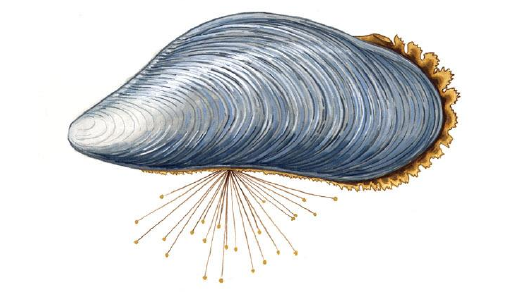
\includegraphics[width=.6\framewidth]{Mussel}
  \end{figure}

\end{frame}

      
    \end{document}
    
    